\chapter{Roleplaying Notes}\label{chap:roleplaying}

\begin{figure}[!htb]
\centering
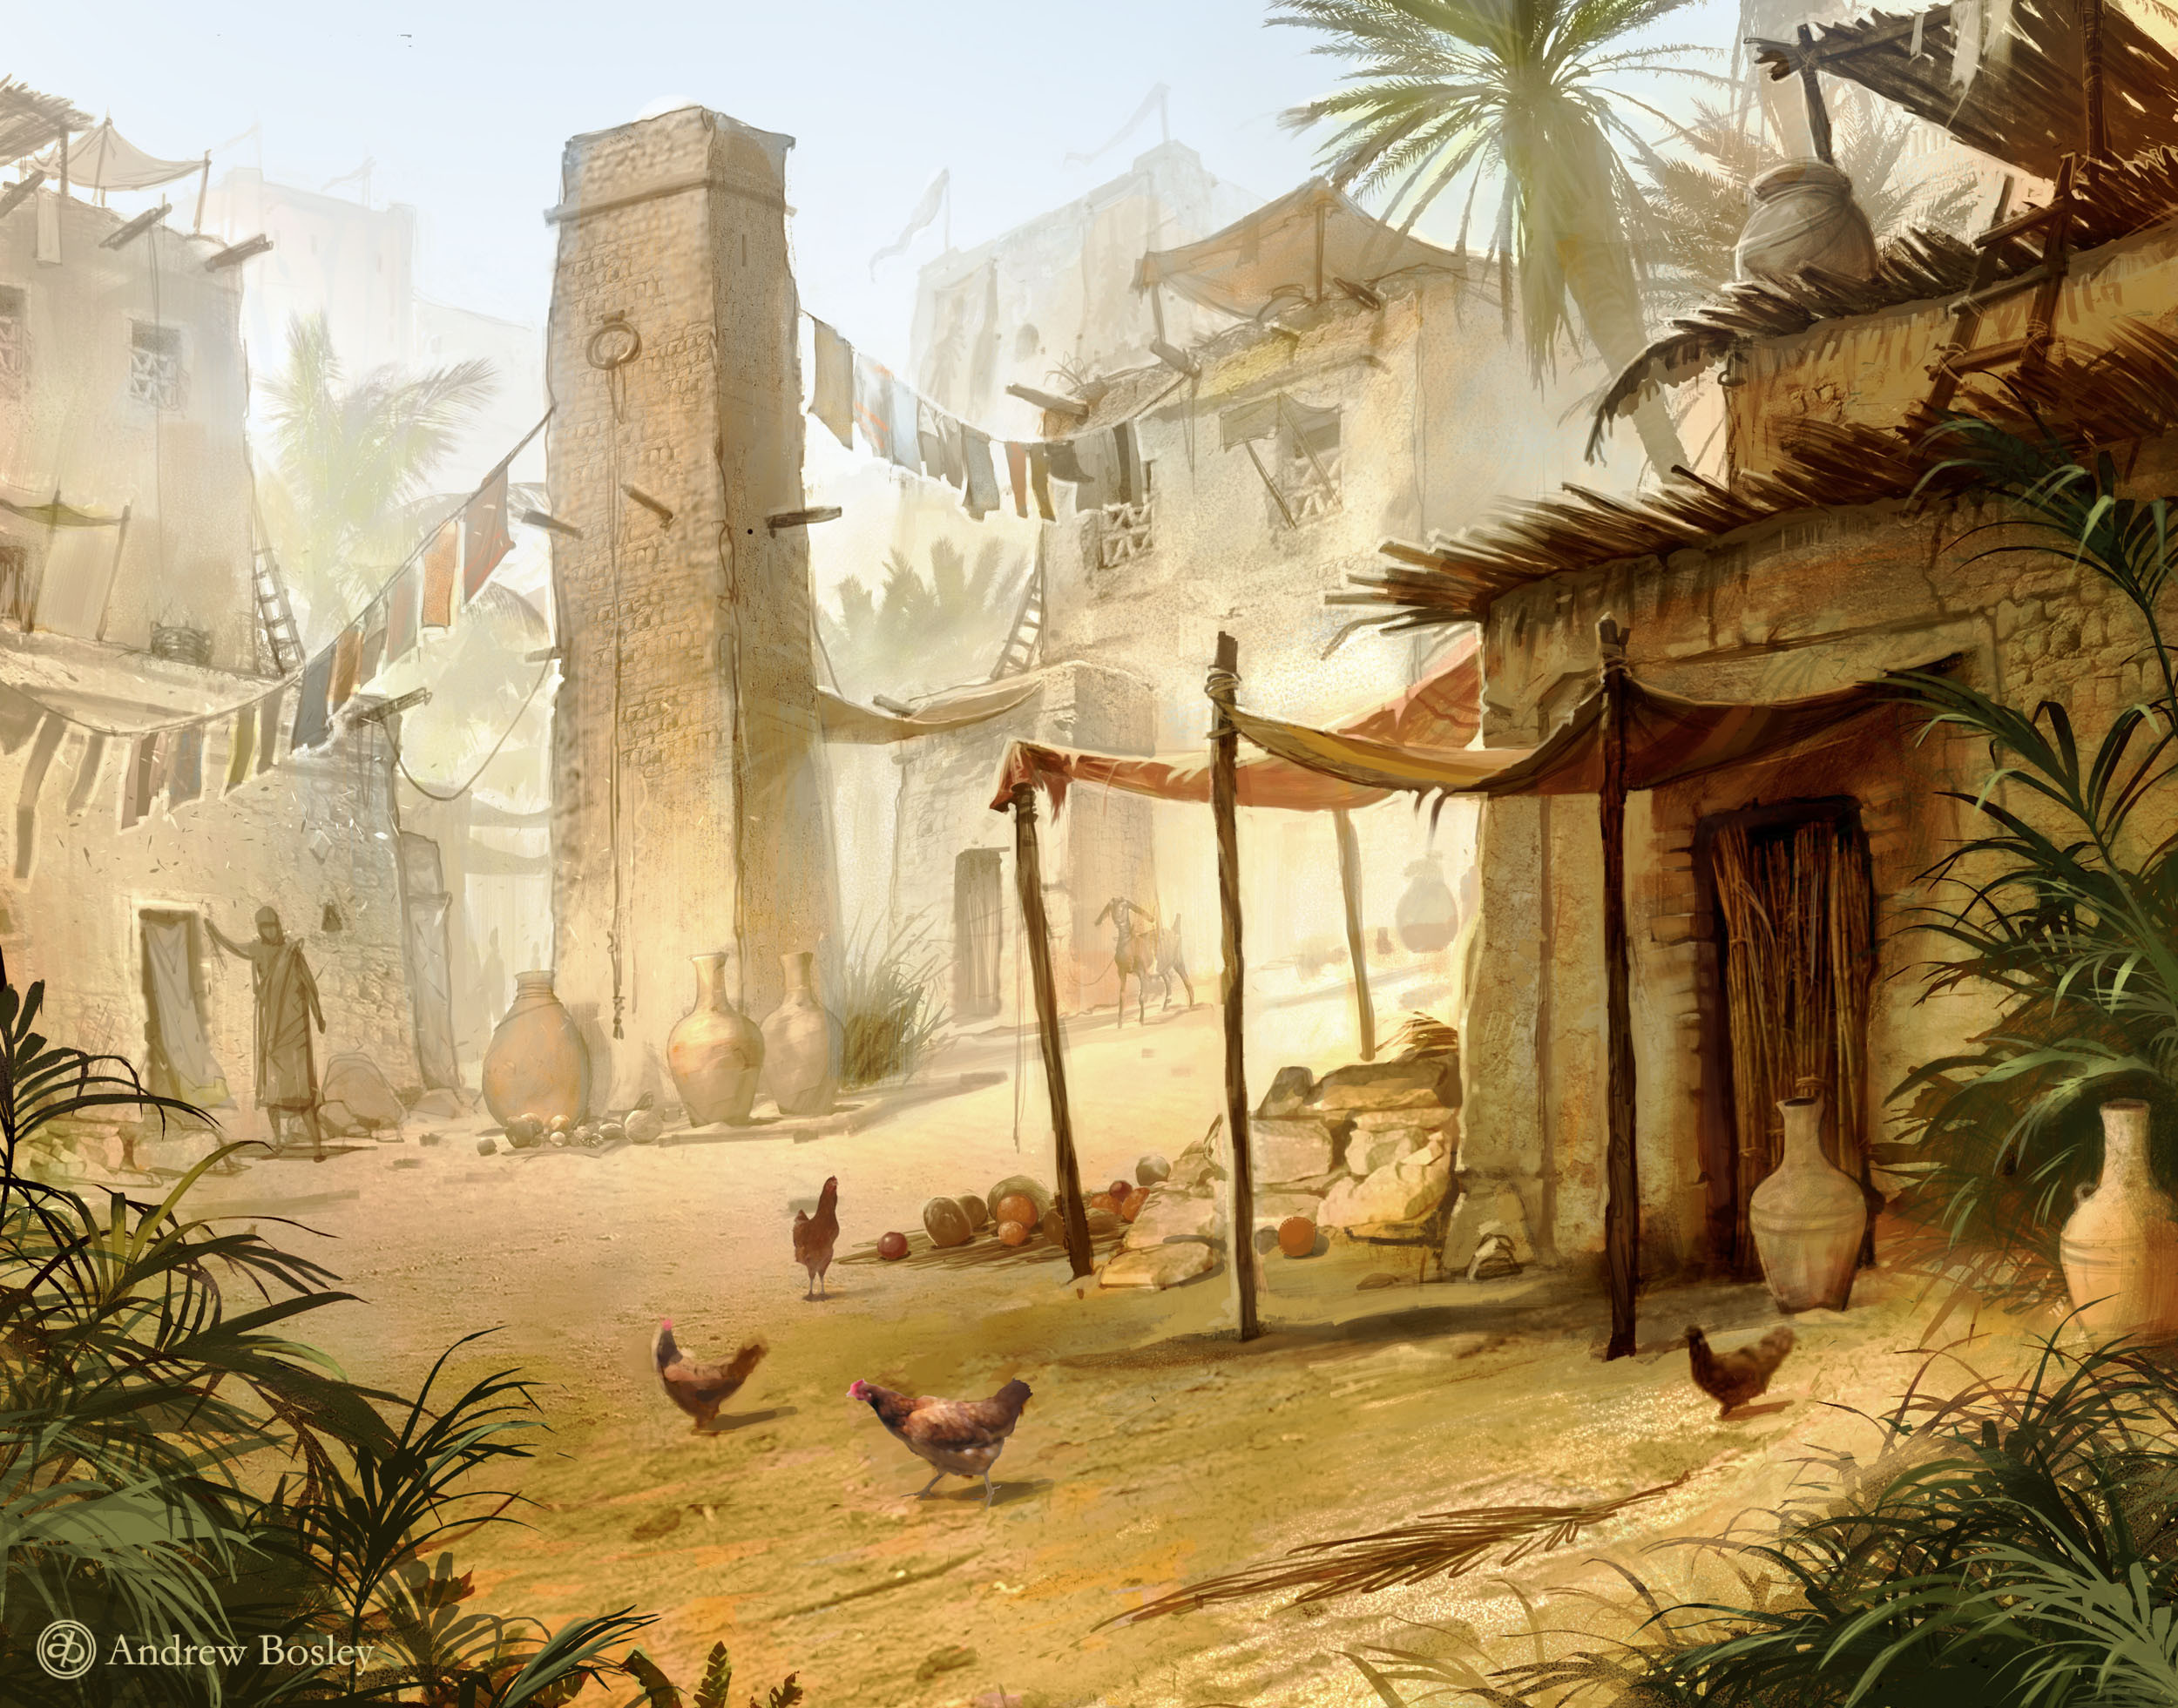
\includegraphics[width=0.7\linewidth]{images/village.jpg}
\end{figure}

\epigraph{\textit{
"I live in a world of fire and sand. The crimson sun scorches the life from
 anything that crawls or flies, and storms of sand scour the foliage from
 the barren ground. This is a land of blood and dust, where tribes of feral
 elves sweep out of the salt plains to plunder lonely caravans, mysterious
 singing winds call travelers to slow suffocation in the Sea of Silt, and
 selfish kings squander their subjects’ lives building gaudy palaces and
 garish tombs. This bleak wasteland is Athas, and it is my home." } } { - The Wanderer’s Journal }

\textit{I've compiled a few lists of things that most characters would know to use as a player handout in my games.
During character creation, hand out each section that applies to each character (race, social class, city state)
as they are chosen, the others that don't get used can be quick reference guides for things like knowledge checks,
or info for when players interact with NPCs and are asking questions.}

\section{General}

\begin{multicols}{2}

\begin{description}
    \item There are no gods.
    \item A full skin or pot of water is worth your life.
    \item You can’t trust an Elf.
    \item Athas is an endless wasteland, spotted by tiny oases, and filled with predators.
    \item The desolate condition of Athas is the result of unchecked magic use.
    \item Arcane spellcasters are mistrusted at best, and reviled more often than not.
    \item The tablelands are dotted with ruins from an ancient past.
    \item Every creature, and even a few plants have some form of latent psionic power.
    \item There are seven city states: Balic, Draj, Gulg, Nibenay, Raam, Tyr, and Urik, each ruled by an oppressive Sorcerer King.
    \item Even more powerful than the Sorcerer Kings is The Dragon, who demands tribute of 1000 slaves from each city state each year.
\end{description}

\subsection{Races}
\subsection{Dwarves}

\begin{description}
    \item Nothing comes before family except your Focus.
    \item A Dwarf’s chief love is toil.
    \item If a Dwarf dies with his Focus incomplete, he returns as an undead Banshee to haunt the objective of his Focus.
    \item Dwarves are hairless and consider the very idea of hair repulsive, though carvings at the Dwarven city of Kled show Dwarves sporting hair and beards in the ancient past.
    \item The three primary Dwarven settlements are North and South Ledopolus, and Kled, a Dwarven village near the City State of Tyr.
    \item The Dwarves of North and South Ledopolis are trying to build a bridge to connect the two villages, but the giants living on Ledo Island in the center keep wading out across the Silt Sea to destroy the bridge.
    \item Dwarves shun arcane magic as a rule, and while they will travel with a spellcaster who proves themselves a worthy companion (by actively working towards the Dwarf’s Focus), they rarely ever fully trust a wizard.
    \item Dwarves who study The Way tend to excel in its use, and many Dwarves become Clerics of Earth, while Fire and Water also tend to attract Dwarven devotees.
    \item Dwarves almost always have a serious, sober demeanor. Only when they’ve completed their Focus do they allow other Dwarves, and their most trusted non-Dwarven friends see their joy and sense of humor (and that lasts only until another Focus is chosen).
    \item Nothing is impossible in the eyes of a Dwarf. The fastest way to earn the enmity of a Dwarf is to tell him “It can’t be done.”
\end{description}

\subsection{Elves}

\begin{description}
    \item \textit{"Death is stillness, so run, you Elves. Dance to the beat of life, for the moment is quick and oh so short. There is nothing as fast nor as proud nor as wonderfully made as an Elf."}
    \item You can’t trust anyone, especially outside your own tribe (until they’ve passed a series of trust tests).
    \item Those that fall behind are left behind.
    \item To ride rather than run is to have no honor.
    \item Of all the races, Elves are the most likely practitioners of sorcery, particularly Defiler magic.
    \item Elves do not usually excel in the pursuit of Psionics, because most lack the dedication to continue their studies.
    \item Elves live for the “now”. They have little care for anything but instant gratification. Looking back the past reminds them of lost opportunities for fleeting happiness, while the future is almost certainly going to be worse than now.
    \item Elves revere Coraanu Star Racer, the Warrior Thief and mythical “first elf” as a pinnacle of Elvishness to aspire to.
    \item Elves will often flaunt a stolen item right in front of its former owner. Elven culture dictates the victim should congratulate the Elf on the possession of such an attractive item. Those who do not are considered poor sports.
    \item Elven chiefs are customarily given a percentage of the gains from any raid. An Elf who holds out on his chief is considered disloyal to his tribe.
\end{description}

\subsection{Halflings}

\begin{description}
    \item Death is preferable to slavery.
    \item Wages are a form of slavery.
    \item Halfling speech is riddled with idioms and cultural references.
    \item Halflings have a very rich and diverse culture.
    \item Halflings are more concerned with how their deeds help improve Halfling culture, rather than amassing great treasures.
    \item Halflings are mainly carnivorous and prefer their meat raw.
    \item Halflings are very concerned with the condition of the environment and will take any measure to keep their jungle from becoming like the rest of the tablelands.
    \item Halflings have little to no concept of conquest and plunder in their culture.
    \item Halflings don’t require as much food or water as the larger races.
    \item Halfling chiefs are much like the Sorcerer Kings of the great city states, but are all Preservers rather than Defilers.
\end{description}

\subsection{Half-Elves}

\begin{description}
    \item Half-Elves pride themselves on their self-reliance.
    \item Most Half-Elven children are usually abandoned by their Elven parent.
    \item Half-Elves almost always have human names, most being unable to earn a proper Elven name.
    \item Half-Elves predominantly live within human society, or out in the wilderness as hermits as they have no separate culture of their own.
    \item Half-Elves readily take to studies and professions that favor solitary independence. Magic, Psionics, and the element of Water all are common pursuits.
    \item Half-Elves also become Druids quite often due to their natural inclination towards solitude.
    \item Half-Elves often find the Templarate a fitting life.
    \item Many Half-Elves resent Elves, yet also feel a need to win their approval.
    \item A Half-Elf is just as likely to seek companionship from an animal as they are from another person.
    \item Due to their heightened senses and the fact that they are usually more reliable than Elves, many Half-Elves are hired by merchant caravans as scouts and outriders.
\end{description}

\subsection{Half-Giants}

\begin{description}
    \item You have no culture/cultural identity of your own, so you readily adopt the culture and behavior of those you admire.
    \item Despite their size and fearsome reputation, Half-Giants tend to possess an almost child like friendliness and curiosity.
    \item Half-Giants also have a ferocious temper, only a fool would tempt a Half-Giant’s rage.
    \item Half-Giants rarely have the patience or mental facilities for learning magic or psionics, though the occasional clever Half-Giant might dabble with Metacreativity or Psychokinesis and become a truly terrifying psychic warrior.
    \item Half-Giants rarely become leaders, more often than not they follow an admired or charismatic friend into adventure, or whomever they find particularly interesting.
    \item Half-Giants require twice as much food and water as other demihumans.
    \item Your large size sometimes causes you to accidentally break human-sized dwellings and furniture.
    \item Most Half-Giants live their lives as slave soldiers, though the more ambitious and adventurous among them sell their services as highly sought after mercenaries.
    \item If you meet someone interesting enough, you might completely abandon whatever it is you’re doing to follow them.
    \item Legend has it a great Sorcerer King created your race long ago.
\end{description}

\subsection{Humans}

\begin{description}
    \item Humans are ubiquitous in the tablelands of Athas.
    \item Humans are the most adaptable among races and fill stations from the lowliest slaves and hermits to the rulers of the great trading houses and high templars of the Sorcerer Kings themselves.
    \item Humans take readily to studying The Way, as well as the worship of the elements.
    \item Most humans distrust and fear arcane magic. Many wizards, both preservers and defilers, have been killed by an angry mob.
    \item There is nothing human ingenuity cannot accomplish.
\end{description}

\subsection{Muls}

\begin{description}
    \item You were born a slave, and you will likely die a slave.
    \item Most Muls are kept as gladiator slaves, due to their nearly unmatched physical prowess.
    \item The life of a gladiatorial slave can be almost as lavish as that of the nobility, if you continue to perform well.
    \item While many Muls have the opportunity to win their freedom many choose to remain in the arenas.
    \item You are stronger than the other races, what would be considered intolerably painful for others is only a mere distraction for you.
    \item Your stamina is unparallelled. You can quarry rock for a full 12 hours with no rest or walk for days without stopping. As long as you sleep at least 6 hours every few days, you don’t suffer from fatigue.
    \item Unlike the Dwarves they are descended from, Muls often sport tattoos, from shoulder markings denoting victory in the arenas to full body tattoos.
    \item Most Mul births result in the death of the mother, especially if the mother is human.
    \item Muls are born sterile and can have no children.
    \item Despite their formidable physique Muls don’t always make good soldiers. They’re smart enough to tell when a commander is making a tactical error, and stubborn enough to refuse such orders.
\end{description}

\subsection{Thri-kreens}

\begin{description}
    \item Elves are tasty.
    \item Humanoid customs are strange, and most of the time none of the other races seem to understand Thri-kreen ways.
    \item Thri-kreen have a pack mentality, and tend to view everything from a predator/prey point of view.
    \item Many Thri-kreen develop psionic powers beyond a simple wild talent, they make excellent Monks and Psionicists.
    \item Some Thri-kreen are capable of delivering a poisonous bite.
    \item Thri-kreen possess great agility and can leap great distances.
    \item Since you do not sleep, you don’t understand why other races seem to become lazy during certain parts of the day.
    \item You live for the hunt, little else interests you.
    \item Thri-kreen have no disposition towards magic, especially arcane.
    \item There are no known Thri-kreen settlements within the tablelands.
\end{description}

\end{multicols}

\section{Caste}

\begin{multicols}{2}

\subsection{Freeman}

\begin{description}
    \item Templars can enter your home at will.
    \item While you are not a slave, you must devote most of your time to earning enough money to keep your freedom.
    \item Most freemen are crafters and artisans, others run market stalls or smaller businesses like taverns and brothels in the less savory parts of the city.
    \item Most freemen own at least a small home.
    \item Very occasionally a freeman is successful (or lucky) enough to rise into the ranks of nobility through sheer wealth.
\end{description}

\subsection{Noble}

\begin{description}
    \item You have been born into a life of luxury, but also one of political intrigue.
    \item You never set foot outside of the safety of your villa or compound without your guards, palanquin to ride in, or at the very least a good disguise.
    \item You have slaves to deal with the things lesser people have to do themselves.
    \item Many nobles have personal bards, consorts, and other “toys” to keep them occupied.
    \item A favorite pastime of the nobility is betting on their favorite gladiator(s).
\end{description}

\subsection{Slave (Artist)}

\begin{description}
    \item You are a slave. You were either born into slavery, could not pay a debt, or were caught committing a crime and were sold into slavery.
    \item Your owner/master may have taught you how to read and write, but this skill is illegal in all of the city states, and will likely get you killed if anyone finds out.
    \item The best way to stay alive is by creating whatever type of art keeps your master happy.
    \item You live a lavish lifestyle for a slave, rivaled only by gladiatorial champions.
    \item Attempted escape carries a penalty of death.
\end{description}

\subsection{Slave (Farmer)}

\begin{description}
    \item You are a slave. You were either born into slavery, could not pay a debt, or were caught committing a crime and were sold into slavery.
    \item To earn your freedom, you have to work off your debt.
    \item When you aren’t working you are sleeping, you have little time for anything else.
    \item If you move your hand to your mouth without permission while working in the fields, you will lose a hand. If it happens again, you will be beaten to death.
    \item Attempted escape carries a penalty of death.
\end{description}

\subsection{Slave (Gladiator)}

\begin{description}
    \item You are a slave. You were either born into slavery, could not pay a debt, or were caught committing a crime and were sold into slavery.
    \item Your purpose is to fight for the entertainment of others, sometimes to the death.
    \item The life of a gladiatorial slave can be almost as lavish as that of the nobility, if you continue to perform well.
    \item You can win/buy your freedom if you are good. If you aren’t, you will likely end up pitted against a superior opponent so that your death can entertain the crowds.
    \item Attempted escape carries a penalty of death.
\end{description}

\subsection{Slave (Laborer)}

\begin{description}
    \item You are a slave. You were either born into slavery, could not pay a debt, or were caught committing a crime and were sold into slavery.
    \item To earn your freedom, you have to work off your debt.
    \item When you aren’t working you are sleeping, you have little time for anything else.
    \item All you know of life is either toiling day in and day out in a mine or quarry, or building something for your master.
    \item Attempted escape carries a penalty of death.
\end{description}

\subsection{Slave (Soldier)}

\begin{description}
    \item You are a slave. You were either born into slavery, could not pay a debt, or were caught committing a crime and were sold into slavery.
    \item To earn your freedom, you have to work off your debt by completing your term of deployed service.
    \item Attempted escape carries a penalty of death.
    \item Most of your life is spent in the training yards, preparing for war.
    \item When battle comes, you can be sure to be placed on the front lines where fighting is the fiercest and mortality rates are staggeringly high.
\end{description}

\subsection{Tribal (can be used in place of both social standing, as well as city state)}

\begin{description}
    \item City states seem claustrophobic to you, everything is too close, there are too many people, and they stink of shit.
    \item Whether a tribe of nomadic herdsmen, hunter-gatherers, or raiders, you are often on the move, never staying put for too long.
    \item You have seen things out in the wastelands of Athas that most people in the cities couldn’t even comprehend.
    \item Most tribes, regardless of vocation, tend to be comprised of a single race. The exception to this, of course, are the tribes of escaped slaves.
    \item In most tribes the leader is the strongest individual, and changes in leadership tend to be violent.
\end{description}

\end{multicols}

\section{City States}

\begin{multicols}{2}

\subsection{Balic (based on ancient Greek and Roman culture)}

\begin{description}
    \item Andropinis claims he was elected to the position of lifelong dictator over 700 years ago.
    \item Templars in Balic are elected for 10-year terms. Andropinis usually makes it clear which ones he favors, and on the rare occasion that the “wrong” one wins, they disappear.
    \item Andropinis’ personal army consists of 10,000 mostly human foot soldiers carrying lances, large wooden shields, and bone daggers (hoplites).
    \item Every citizen of Balic is a member of the militia and spends every 10th month assisting the regular army patrol the fields to reduce crop and stock loss to Giants who regularly raid from across the Silt Sea.
    \item Balic is situated in the Estuary of the Forked Tongue, a very defensible location as far as invasion from the other city-states is concerned, as it is surrounded by parts of the Silt Sea on the North, East, and South sides.
    \item Balic has a strong economic district, which specializes in trade of olive oil, kank nectar, and pottery.
    \item The Agora, or market square is completely ringed in by the Elven market, making it impossible to do any legitimate business without dealing with the dubious offers of the Elven merchants.
    \item The Silt Sea contains numerous islands inhabited by giants, and dotted with crumbling ruins.
    \item Shipfloaters are psionicists who telepathically levitate ships to traverse the Sea of Silt.
    \item \textbf{Rumour:} The Dwarves of North and South Ledopolis are trying to build a bridge to connect the two villages, but the giants living on Ledo Island in the center keep wading out across the Silt Sea to destroy the bridge.
\end{description}

\subsection{Draj (based on Aztec culture)}

\begin{description}
    \item The Mighty and Omnipotent Tectuktitlay, Father of Life and Master of the Two Moons claims to be a living god.
    \item Templars in Draj are known as Moon Priests.
    \item The fertile soil surrounding Draj allows it to grow many crops, including grain for bread and hemp, which makes for good ropes.
    \item Draj is almost constantly at war, raiding villages and even other city states for captives to be sacrificed on the steps of Tectuktitlay’s pyramid, overlooking the gladiatorial arena.
    \item Knowledge of history is expressly forbidden by Tectuktitlay, nothing beyond mortal memory is really known about the past of this city.
    \item Draji warriors decorate themselves with the skins of various beasts and animals, and carry obsidian-edged clubs called Macuahuitl as well as short harpoons.
    \item Criminals in Draj receive only one sentence: death, either by execution or by caging (a very slow death by exposure).
    \item Crime, especially theft is so looked down upon by Draji culture that most citizens would rather sell themselves into slavery than steal.
    \item Instead of a wall, the entrance to the city state is surrounded by expansive mud flats, which provide plenty of protection from invaders.
    \item \textbf{Rumour:} Draj has vast storehouses of grains and hemp that it keeps hidden from everybody in order to drive up their prices when trading with other city states.
\end{description}

\subsection{Gulg (based on various African savannah cultures)}

\begin{description}
    \item Lalali-Puy, the oba, or forest goddess is the only ruler of a city state who enjoys the popular support of her people.
    \item Gulg lies at the southern end of the Crescent Forest.
    \item Nearly everything in Gulg is made from Agafari wood, even the houses are carved out of the very trees.
    \item Lalali-Puy controls all economic activity within Gulg directly, taking all the food produced and distributing it amongst her people. Merchants from outside the city can trade with the city state, but it is forbidden to trade with the citizens themselves.
    \item Citizens of Gulg also have the right to appeal directly to Lalai-Pui for an audience if they need a matter resolved.
    \item Gulg’s city wall is a magically infused hedge of thorny brambles that actively seek out the flesh of those who try to penetrate it.
    \item Despite what the title of city state invokes, Gulg is actually a collection of villages all crammed together within the shelter of the city wall.
    \item When a new Nganga (templar) is chosen, the district they come from holds a funeral service to symbolize that the citizen they once were is no more.
    \item The templars of Gulg wear masks or face paint to hide their features and strike fear into those who would oppose the Oba.
    \item \textbf{Rumour:} If not for the power of the Oba and her Judagas (warriors), Nibenay would likely have destroyed or taken Gulg over long ago.
\end{description}

\subsection{Nibenay (based on Angkor culture)}

\begin{description}
    \item Nobody can remember the last time Nibenay, the Shadow King was seen outside the Naggaramakam.
    \item The Naggaramakam is a walled central district in which only Nibenay’s Templars may enter and leave. Slaves who enter here are never permitted to leave again.
    \item Nibenay lies at the northern end of the Crescent Forest.
    \item Every surface of every building in Nibenay is covered with carvings of various figures.
    \item Nibenay holds the only permanent Elven market, which is run by the Sky Singers tribe.
    \item The Monastery of the Exalted Path is an all male psionics academy, the female counterpart is called The Monastery of Serene Bliss. Both are well respected.
    \item A line of large statues of King Nibenay stand on each side of the main road to the city. The statues are called the Omnipotent Receivers as it is believed that the Shadow King can see through their eyes.
    \item Some people believe that the Shadow King hasn’t been seen because he actually died a long time ago.
    \item All Nibenese templars are female and are sometimes referred to as Nibenay’s Wives.
    \item \textbf{Rumour:} the ruins of Giustenal are said to contain a powerful psionic entity.
\end{description}

\subsection{Raam (based on ancient Indian and Egyptian culture)}

\begin{description}
    \item The Great Vizier Abalach-Re claims to be the emissary of a higher power known as Badna.
    \item Abalach-Re assures citizens that Badna watches her closely and will strike her down if she falters in her duties, but few believe her.
    \item Almost no citizens of Raam actually respect their Sorcerer Queen, and there is open talk of rebellion in the streets.
    \item The nobles of Raam are little more than warlords constantly fighting against each other and jockeying for position in the inevitable revolution.
    \item Templars of Raam almost never travel alone, lest they are murdered in the streets.
    \item Raam culture consists of a rigid caste system.
    \item While it was once an economic powerhouse, and still remains the largest city-state on the tablelands, Raam’s infrastructure has fallen almost completely apart due to the indifference of Abalach-Re who prefers to take pleasure in whatever strikes her fancy rather than rule her city.
    \item Crime runs rampant in the streets without the presence of templars to maintain order.
    \item Abalach-Re has born hundreds of illegitemate children over the 30 or so generations that she has ruled Raam. Known as the Offspring, many of her children have exhibited unusual psionic and arcane talents.
    \item \textbf{Rumour:} Stay away from the ruins of Yaramuke. Hamanu of Urik used such foul magics to destroy it that the entire area, including the fresh water springs that flow from within are all posionous.
\end{description}

\subsection{Tyr (based on the culture of Tyre)}

\begin{description}
    \item King Kalak, the Tyrant of Tyr has allocated an inordinate number of slaves towards working to build his ziggurat, including those owned by the nobility.
    \item Even the iron mines, upon which Tyr’s economy is based have been shut down to allocate more resources to the ziggurat.
    \item Nobody knows what the ziggurat is for.
    \item Kalak’s Templars as well as his personal guard are all armed with iron swords.
    \item As in most of the city states, while Tyr’s Elven Market is always in the same area, the vendors are always changing from one day to the next.
    \item Because most of the slave laborers have been working on the ziggurat, the remaining gladiatorial slaves have been putting on more and more impressive fights, rather than the barbarically uneven matches that were normally seen before. This in turn is increasing the draw that the games have to the point where seat prices have risen dramatically.
    \item People are starting to whisper that King Kalak has gone mad.
    \item Tyr is located in a valley along the edge of the Ringing Mountains.
    \item Taxes have also risen dramatically since Kalak began the construction of his ziggurat.
    \item \textbf{Rumour:} Tyr was built atop the ruined foundations of an ancient city. Though many of the passages and byways are blocked off either by more recent construction, or shifting dunes, there are still many hidden access points to various locations under the city. This area is known as UnderTyr.
\end{description}

\subsection{Urik (based on Babylonian culture)}

\begin{description}
    \item King Hamanu trains daily with his warriors, even the slaves.
    \item The walls of Urik are famous for being nearly unbreachable.
    \item You would do well to remember all of Hamanu’s many laws if you don’t want to find yourself being sold into slavery by a templar.
    \item Urik lies near the Dragon’s Bowl - a massive crater with 1000 foot high cliffs leading down to a large lake in the bottom.
    \item The majority of the tools and weapons found in Urik are made from obsidian, which is mined from the nearby Smoking Crown mountains.
    \item Statues of lions top the massive walls, where guards patrol with their bows and obsidian-tipped arrows.
    \item Urik’s gladiatorial arena, known as the Pit of Black Death, rests in an old abandoned obsidian mine, its walls lined with razor sharp obsidian.
    \item Children are tested by templars at an early age and are assigned a vocation based on their abilities. It is extremely rare for a change in career in Urik.
    \item Children who show talent in The Way are taken from their parents and sent to Hamanu’s school of the mind for training.
    \item \textbf{Rumour:} King Kalak of Tyr has stopped production of iron, Hamanu might send his army to get more iron!
\end{description}

\end{multicols}

\section{Dark Sun Food}

\subsection{Drink}

\begin{multicols}{2}

\subsubsection{Non-Alcoholic}

\paragraph{Filtered Jalath’gak-blood Nectar} Another sweet nectar.\\
\paragraph{Kank Honey} This sweet liquid is produced in globules on the abdomen of the large insects.\\
\paragraph{Kola Tea} Kola nuts are from Gulg. The nuts can be grounded into a fine powder which is then steeped in water. The resulting beverage is tasty and also stimulates the mind and wards off sleep.\\

\subsubsection{Alcoholic}
\paragraph{Ale, General} Raam and Tyr both export ale. Cheap ale is served warm.\\
\paragraph{Asticles Wine} Asticles wine has a pale golden color and a tart, dry scent. It has a light taste that leaves the mouth dry. It is a very fine drink and as such is very expensive. Asticles wine is the preferred drink of nobles in Tyr.\\
\paragraph{Beer} Gulg exports beer. Cold beer is available but expensive.\\
\paragraph{Brown Wine} Brown wine is thick and is an acquired taste.\\
\paragraph{Broy} Broy is made from fermented kank nectar. Spiced broy and watered-down broy are also available. When served plain, it is potent and foul tasting. However, broy can be served warm and spiced with a pungent herb that disguises its sourness, as well as enhanced its enrapturing powers.\\
\paragraph{Bulis Berry Wine} The bulis berries can be made into a wine with a dark blue-purple color. The taste is sickeningly sweet and so is often mixed with water. It is rather inexpensive and is mainly purchased by working-class Athasians.\\
\paragraph{Cactus Blue Ale} Cactus blue ale is served in Tyr and is made from fermented grall. The ale has a strong, rough taste and is very potent.\\
\paragraph{Cider} Gulg exports cider.\\
\paragraph{Elven Wine} Many elven tribes make their own wine, thought the process and quality vary from tribe to tribe. The Fastcoin elven tribe specializes in the sale of a simplistic elven wine, light on taste but fast and cheap to produce. Sky Singer wine, on the other hand, is made from kank honey and is an acquired taste, potent in both flavor as well as alcohol content.\\
\paragraph{Goat’s Milk} Fermented goat’s milk is served in bars.\\
\paragraph{Honey Barley Ale} Honey barley ale is made from honey barley. It has a smooth taste that is slightly sweet.\\
\paragraph{Javo Nectar} Fermented javo nectar is potent. The nectar retains the sweet flavor of the javo, but does not have the obnoxious smell.\\
\paragraph{Klick-win} Klick-win is a sickly-sweet wine made from fermented flowers by tohr-kreen. It is not usually available in the Tablelands.\\
\paragraph{Milkwine} Milkwine is a gummy liquid.\\
\paragraph{Palewater Ale} Palewater ale is served in Salt View. It has a rough yet simple taste.\\
\paragraph{Palm Wine} Palm wine is of poor quality but is affordable to the lower classes.\\
\paragraph{Port} Good port is available. A sweet dessert wine, it is drunk exclusively by the nobility.\\
\paragraph{Pulque} Pulque is fermented cactus juice that is drunk in Draj. Pulque comes from the huge maguey cactus. The taste is milky and slightly sour.\\
\paragraph{Red Wine} Thick red wine is served in Tyr.\\
\paragraph{Sapwine} Sapwine is tart. It is fermented from tree resin and has a powerful kick. Most consider it to be the foulest drink available in the wine shops of Tyr and Gulg.\\
\paragraph{Scuppernong Wine} Scuppernong can be fermented into a silver wine that is thick, with a slightly bitter taste. Scuppernong is the favored drink among elves.\\
\paragraph{Spiced Mead} Spiced mead is served in many taverns.\\
\paragraph{Spiced Wine} Spiced wine is sold in wine shops. The wine is mixed with a variety of spices to give it a strong flavor.\\

\end{multicols}
\hrulefill

\subsection{Meats}

\begin{multicols}{2}

The various meats that make up an Athasian's diet can be prepared in a variety of ways. In the city-states the most common methods of preparation are bite-size bits on a skewer cooked over an open flame, or a slab or steak grilled. For journeys across the desert or the Silt Sea, meat is either smoked or dried and preserved in salt. However, only rich merchants and caravan captains are served the prepared meat; the rest of the caravan is typically fed a stew using the leftover scraps of meat.

\paragraph{Aprig} Aprig meat is succulent and has a faint nutty flavor.\\
\paragraph{Boneclaw, Lesser} One lesser boneclaw provides 11kg of meat. Each lesser boneclaw has a fluid sac on its back which contains about 1.5l of water but is tainted by the boneclaw's.poison.  Creatures drinking the water unpurified are affected by an ingested version of the lesser boneclaw poison. \\
\paragraph{Boneclaw, Greater} A greater boneclaw can be eaten but the meat is tough and stringy. One greater boneclaw provides up to 60kg of meat.\\
\paragraph{Carru} One carru can provide 100kg of meat for consumption. Carru is a red meat. Wild carru meat tends to be much leaner than that from domesticated carrus, which is fatty and has more flavor. All carru have a fluid sac behind their heads which contains about 3l of water.\\
\paragraph{Chafthrang} The meat of a cha-thrang is very expensive and only eaten by nobles on those rare occasions when it is available. The meat must be specially prepared to ensure that the toxic lime from the creature's shell is removed before cooking. The meat is very tough, making it difficult to eat in large chunks, and thus it is typically ground up and added to stews and soups.\\
\paragraph{Cloud Ray} The meat of a cloud ray is very expensive and rare. A single cloud ray could easily provide an entire settlement with enough meat for 2 to 3 months.\\
\paragraph{Crodlu} Crodlu meat is tough and stringy. Some enterprising cooks have found ways to use the meat in stews and other dishes to compensate for its texture. One dish involves ground crodlu meat mixed with rice.\\
\paragraph{Erdlu} Erdlu meat is very common and often used in stews as well as grilled. The meat does not need to be fully cooked to be safe to eat, and so can be prepared medium rare. It has no aftertaste. In Draj, some popular dishes include erdlu stew and steamed corn; a dried, pemmican-like erdlu meat that is part of the local diet; and spiced erdlu meat with vegetables.\\
\paragraph{Erdland} The large erdlund provides up to 300kg of meat and tastes similar to erdlu.\\
\paragraph{Fish} Fish is the rarest of delicacies in the cities of the Tablelands. Only the riches nobles and templars have tasted fish flesh. The fish are typically farmed in specially maintained pools for the exclusive enjoyment of their noble owners.\\
\paragraph{Gorak} Gorak meat is common quality and leaves a strong, greasy aftertaste.\\
\paragraph{Inix} An inix can provide a lot of meat, but most if it is considered average quality because it is lean and tough. The tail meat of an inix, however, is considered a delicacy. Despite the quality, inix meat is very versatile and used in a variety of dishes. In Tyr, inix meat is fried. Fillet of inix in a spicy sauce is a dish served in Raam. The meat can be added to a rich stew as is done at banquets for nobles in Raam.\\
\paragraph{Jankz} The meat has a gamey taste but is palatable. Because of the poison sacs, caution must be taken when preparing jankz. As a general rule, one jankz provides a meal for one man.\\
\paragraph{Kip} Kip meat is fatty and greasy. Kip sausages are served with biscuits in Tyr, while kip meat is a staple of many dwarven communities. One kip can provide meat for up to 2 meals. The meat of one kip can also be made into a stew that willd easily feed six.\\
\paragraph{Kirre} Kirre meat is considered some of the finest available in the Tablelands. This has lead to over-hunting that has wiped out the kirre in the Crescent Forest, making the meat very difficult to obtain.\\
\paragraph{Kitsu} Kitsus are small bird-lizards. Their meat is tasty but dries quickly if overcooked.\\
\paragraph{Lizard, General} There are numerous types of small lizards used for nourishment throughout the Tablelands. Lizard meat is most often used in spicy stews. Small lizards live in the rocky badlands and foothills of the Ringing Mountains and can provide a meal for a desert traveler. Sweet lizard meats are sold at the arena in Tyr.\\
\paragraph{Mekillot} Mekillot steak is a stable for nobles and rich merchants. It is rich and juicy and typically prepared in thick cuts. In Raam, mekillot steak in a wine and berry sauce is served at banquets for nobles and other powerful figures.\\
\paragraph{Rat} Rats are found in the wilds and in every city-state of the Tablelands. The slaves and the very poor will often trap them for their meat.\\
\paragraph{Renk} Renks are small slugs that are eaten raw. Each slug has four ounces of water within it. When consumed raw each renk provides the equivalent of a . cup of water. An active man would need to eat 32 renks a day to replace his water requirement for the day.\\
\paragraph{Rotgrub} Fried rotgrubs are served in the bazaars of many cities.\\
\paragraph{Silt Crab} Silt crabs live on the shores of the Sea of Silt. Most species are the size of a man'fs fist. They must be boiled in water before eaten; otherwise a toxin is released into the crab's flesh when it is killed.  While the toxin is not strong enough to kill a character, eating more than a couple of the crabs in this way would cause the victim to become violently sick and regurgitate any food they had recently consumed.\\
\paragraph{Silt Mussel} These mollusks live in the Silt Sea. They have an oblong shell, about an inch long, that must be cracked or pried open to get to the meat inside. Silt mussels can be eaten raw, but the taste is very dry and gritty due to their silty environment. In most city-states they are boiled in water. In Raam silt mussels are served with a peppery sauce.\\
\paragraph{Silt Spawn} Silt spawn meat is tasty and can be used as a source of food. Giants hunt silt spawn for food and consider them a delicacy.\\
\paragraph{Silt Serpent} The giants and others who live along the shores of the Sea of Silt know that silt serpents make excellent meals. Their meat is sweet, tasty and extremely juicy, and it can be eaten raw or cooked over a slow-burning fire. The Sky Singers elf tribe makes a particularly famous dish using silt serpent meat and faro leaves. The meal, called alrasb in elven can be sampled in Nibenay'fs Hill District or the food tents of the Sky Singers' roadside bazaars.\\
\paragraph{Snake} Athasians include a variety of snakes in their diets. In cities snakes are usually cooked on skewers, chopped into round slices with the skin still on.cooks claim this helps to keep in the flavor. Whether true or not, the skin must be removed before eating. Harmless, albino snakes can be found amongst the crags and foothills of the Ringing Mountains. These snakes can provide a safe meal for a desert traveler.\\
\paragraph{Sygra} The meat of a sygra is palatable but unnoteworthy.\\
\paragraph{Z'tal} The meat of a z'tal is dense and coarse.  The tail and hind legs make excellent eating and are considered the choice portions. The tail and legs are often roasted and can provide up to six meals. Z'tals can be used to prepare a stew. One z'tal can provide enough meat for a stew that would feed 12 people.\\

\end{multicols}
\hrulefill

\subsection{Eggs}

\begin{multicols}{2}

\paragraph{Erdlu Egg} Erdlu eggs have a wrinkled, leathery shell, but are delicious and also nutritious. When eaten raw, the red yolks have a zesty, gamey taste that is both satisfying and invigorating. The whites form a spongy cake that tastes like cheese when cooked. If eaten raw, the egg can take the place of a day's water requirements, but only for up to a week's time. The egg is an excellent source of nutrition, and can keep a man alive for months at a time as the eggs are packed with a variety of nutrients and essential vitamins. If eaten raw an egg can replace 4l of water. However, it is not a perfect substitution and a man can only live on this egg-water diet for one week before he needs water.\\
\paragraph{Erdland Egg} Erdland eggs are less tasty than erdlu eggs, but are large enough to provide food for three men; the eggs are three feet in diameter.\\
\paragraph{Gorak Egg} Gorak eggs are delicious and oft-sought after. The shell is leathery but not as tough as an erdlu egg, making them more fragile. The brown yolks provide most of the flavor while, the whites are soft and spongy.\\
\paragraph{Jalath'gak Nectar} The abdomen of a jalath'gak yields 60l of water. It also yields blood and nectar that can be filtered to provide 32 meals.\\
\paragraph{Kank Honey} Kank meat cannot be eaten; when a kank dies its flesh emits an odor so foul that not even a starving man can stomach it. Food-producer kanks create a melon-sized, honey globule that is very sweet. The honey is thick, green, and provides the eater with plenty of energy. Kank honey is very nutritious and can sustain a man for several days with no other means of nourishment.\\
\paragraph{Kes'trekel Egg} In Nibenay the eggs of a kes'trekel are a delicacy, but only if procured and eaten within two weeks of being laid.\\
\paragraph{Pulp Bee Honey} Worker pulp bees produce a sweet tasting liquid that is very nutritious. One quart of the liquid can provide a human with enough nutrients for two days. The honey hardens into resin a day after been produced. When it hardens the honey looses some of its nutritional value but can still provide the nourishment of one day's food.\\
\paragraph{Pterrax Egg} The eggs of pterrax are a very valuable source of food for those dwelling in mountainous regions. The eggs are almost two feet in diameter and one pterrax egg provides up to two meals.\\
\paragraph{Wezer Honey} Wezers produce a honey on which they feed. Although not the most delectable of the various honey's available to Athasians, its unique flavor and rarity makes it an expensive delicacy.\\

\end{multicols}
\hrulefill

\subsection{Fruits and Vegetables}

\begin{multicols}{2}

Unless otherwise noted, all fruits ripen only once per year, near High Sun, and may be scarcer during the rest of the year. Only in the Forest Ridge and Crescent Forest do fruits ripen more than once per year. Vegetables, on the other hand, are readily available throughout the year. For desert travelers, most of the plants found in the Scrub Plains are safe for humans to eat, but halflings and dwarves should avoid eating anything with purple spots as these cause feverish deliriums and terrible stomachaches.

\paragraph{Agafari Nut} The nuts of the large agafari tree are edible.\\
\paragraph{Baobab Gourd} The gigantic baobab tree produces a gourd-like fruit that is edible. Some species have a sour taste.\\
\paragraph{Bergo} The bergo fruit grows on a tree. The bergo is pear-shaped and has red skin covered in soft green spines. The interior is yellow and contains many tiny seeds; the seeds are about the size of a sesame seed and are edible. The taste of a bergo is mildly sweet and the texture is crunchy due to the seeds.\\
\paragraph{Berill} Berill is a blue-green moss that often carpets the soil of the Crescent Forest. In open clearings the moss dries to a thin shell which crackles when stepped upon. In this state it is edible and tastes like dried tea leaves.\\
\paragraph{Berries, General} Various berries gathered from the Crescent Forest are part of the Gulgan staple diet, including blackberries, blueberries, mulberries, and raspberries.\\
\paragraph{Betel Nut} Betel nuts are eaten by most citizens of Nibenay. Eating the nuts over the years stains the teeth. The Nibenese also grind the nuts into tasty pastes.\\
\paragraph{Broy Bean} Broy beans take their name from the drink, but have little in common with broy. The flat, dull yellow beans taste horrible, reminiscent of bad broy. However they taste, the beans are a big source of protein for those desert communities lacking large animal herds.\\
\paragraph{Bulis Berry} Bulis berries have a hairy, thick brown skin, making it difficult to peel. If one has the patience to peel off the thick skin the small purple center can be eaten and has a sweet, flowery flavor.\\
\paragraph{Cabra} Cabra melons are thick-husked fruits that have a succulent taste. The inside of a cabra melon has wedges similar to an orange.\\
\paragraph{Cactus, General} Many variety of cacti can be eaten. Cacti are most often eaten raw, although some varieties are cooked. Honey-boiled cactus is served in the elven market in Nibenay.\\
\paragraph{Cactus, Prickly Pear} The prickly pear is a red fruit from the prickly pear cactus. It is sweet, but care must be used when peeling the skin because of the hundreds of tiny needle-like spines. The prickly pear is a popular choice to make candy or other snacks involving fruit pulp.\\
\paragraph{Cactus, Red} Red cactus is a round succulent plant with spiny thorns, about the size of a man's head. The cactus is typically used to harvest red cactus grubs, but the fruit of the cactus can also be eaten.\\
\paragraph{Cactus, Rock} A rock cactus can be peeled if it is first incapacitated. Each rock cactus provides approximately 0.5kg of food. The taste is vaguely similar to apples. In addition, a rock cactus provides up to 2l of water.\\
\paragraph{Cactus, Spider} Inside of a spider cactus is 4l of a honey-like liquid similar in consistency to an erdlu egg. Each cactus contains 1l of the liquid, which can be substituted for either food or water. One liter can replace 1l of water or provide nourishment for four meals.\\
\paragraph{Chadnut} The chadnut is sweet. People place them in their mouths and suck on them to get the flavor. The seeds of the chadnut are peppery, burning the tongue and making the eyes water. The seeds leave a fiery aftertaste in one's throat.\\
\paragraph{Copra} Copra is dried coconut. The city of Gulg exports a lot of copra throughout the Tablelands.\\
\paragraph{Corn} In Draj, large fields of corn are grown and is a main stay of the Draji diet.\\
\paragraph{Date} Dates are a delicacy that are enjoyed as a snack or appetizer by the upper classes. For the desert traveler, dates can be a life saver, as dates grow on palm trees that often surround an oasis.\\
\paragraph{Dem Bush} Dem bushes are not very tasty, but they do provide nourishment to a desert traveler. They grow in Rocky Badlands, especially near the Ringing Mountains.\\
\paragraph{Faro} Faro is a dwarf cactus tree, as tall as a man, with a handful of scaly stems that rise to a tangled crown of needle-covered boughs. The twisted cactus grows a blossom that blooms delicious fruit only once per decade. Faro blossoms have a sweet scent and have huge red flowers on the rare occasion that they bloom. Faro is a cash crop. Each piece of sweet fruit is a delicacy worth more than the plant itself. More common uses are found for the needles of the faro. The faro needles can be ground into flour for bread and are also a common ingredient in stews. The needles are made into a gruel for slaves. On many a voyage across the Silt Sea, the galley slaves eat moldering faro.\\
\paragraph{Fig} Figs are a pleasant snack for those who can afford it. The city of Nibenay cultivates fig groves in the Crescent Forest that provide most of the figs available in the cities of the Tyr region. Fig trees often surround an oasis in the desert, providing much needed nourishment to the desert traveler.\\
\paragraph{Geja} Geja is a soft-skinned fruit which is only ripe for a few days each year. It is sweet and delicate. Geja can be dried in the sun, and retains its sweetness when dried.\\
\paragraph{Gourd} The two most common gourds found in the Tablelands are the tulifer and the cucurbata. Tulifer looks like an oval, orange melon with green horns or spikes. The yellow-green flesh is soft and gel-like. If eaten raw it tastes very sour and salty, but if allowed to ripen the sourness is not as strong. The cucurbata is large, over a foot in diameter. It is reddish-brown in color, with a warty exterior. The white flesh is crunchy and watery but becomes bitter as it ripens. When fully ripe the flesh softens and takes on an orange color; by that point the gourd is too bitter to eat.\\
\paragraph{Grall} Grall is a squat, thorny cactus that is eaten raw, though it tastes bitter.\\
\paragraph{Gyava Berry} Gyava berries grow on short, creeping shrubs that resemble vines. The slender, wiry stems have small, sharp leaves. The tiny berries are less than a quarter-inch in diameter and are bright red when ripe. The gyava berries are sweet but have a strongly acidic taste. The berries can be crushed for fruit juice or made into dyes.\\
\paragraph{Javo} Javo is a large oval fruit with a thick brown skin covered in spines, similar to a pineapple. It is the smell of javo that everyone remembers.the smell is a horrible cross between excrement and onions that is detectable from half a mile away when the fruit is fully ripe. Because of the smell, most of the city-states have banished the cultivation of javo to isolated client villages. The inside of the javo is very soft, and contrary to the revolting aroma of the fruits' outer shell, the custard-like interior is nutty and sweet.\\
\paragraph{Junnfruit} Junnfruit has a tough orange rind, but inside it is meaty and juicy. It is eaten by nobles and rich merchants, the only ones who can afford it as a sweet snack.\\
\paragraph{Jute} Jute is a fibrous plant with shiny green leaves. The leaves are often eaten in Raam and Gulg but have a slimy taste. Sometimes the slimy taste is counteracted by adding a large pinch of salt.\\
\paragraph{Kola Nut} Kola nuts are from Gulg. Chewing on kola nuts too much stains the teeth and lips brown and gives one's breath a bitter tang.\\
\paragraph{Neep} Neep is a thick-rooted vegetable with an orange color and a bland flavor. It is often mixed with other food when eaten.\\
\paragraph{N'ku'ru'ma} N'ku'ru'ma are finger-sized pods with short, fine needles. The needles are removed before roasting. The cooked n'ku'ru'ma has a slightly sweet taste.\\
\paragraph{Oleracea} Oleracea is a succulent leafed plant. It is a staple vegetable of most diets. The oleracea has dull yellow, finely incised leaves. It is eaten raw or cooked, but is flavorless in either case.\\
\paragraph{Olive} Balic maintains large olive orchards. The olives can be eaten and are often used to make olive oil.\\
\paragraph{Orange} The Dictator Andropinis of Balic maintained a private orange grove outside his palace. Originally for his pleasure only, the merchant-house of Wavir now sells a limited number of the oranges at a high price.\\
\paragraph{Pepper} To add a dose of fiery spice to dishes, the Draji cultivate both red and green peppers. Their fierce taste is shunned by many who do not understand why the Draji would want to eat something so hot in Athas's scorching environment, but they are still popular with many.\\
\paragraph{Pree Stick} Pree sticks come from a thick, salt-crusted, leafy plant that grows in saltwater. The leaves are baked in the sun to create a crispy salty snack. \\
\paragraph{Scuppernong} The scuppernong is a hearty, rough-skinned silver berry that grows on small shrubs.\\
\paragraph{Silt Weed} Silt weed grows along the coastline of the silt sea. Some rare varieties are edible.\\
\paragraph{Silverbush} Silverbush is a desert plant that stores water in its trunk as a milky sap. It is edible but has a bitter taste. Hot spices are often added to make it more palpable.\\
\paragraph{Soybean} Roasted and salted soybeans are a cheap snack for the spectators in the arena in Nibenay. Soybeans are also added to vegetable dishes to make them more filling.\\
\paragraph{Tarange} Tarange is a nice, sweet fruit, slightly tangy in flavor. There are many varieties of this pear-shaped fruit, though the skin is not edible like that of a a pear. The color of the skin varies by type with colors that range from purple to orange. The center pith is full of inedible seeds.\\
\paragraph{Thornberry} Thornberries are tiny orange berries about a quarter of an inch in diameter. They are soft and juicy. Unfortunately, harvesting thornberries is very difficult as the thornberry bush has long, thin leaves studded with sharp thorns. The berries also have a sharp thorn on their underside that must be removed before they are consumed. Because of the difficulties in harvesting the berries, many farmers crush the berries whole to make juice and then later filter out the thorns. Thornberries are most commonly sold in the arena in Tyr.\\
\paragraph{Tubers and Roots} Tubers and roots are a large part of the diet of most desert communities. The most common tuber is the solanu, a sturdy brown tuber that is marked above ground by hairy stems sprouting large leaves. After it is peeled, the solanu can be eaten raw, dried, or cooked. The flesh is white, and a woody pit, slightly yellow in color, runs down the center. The flesh darkens quickly when exposed to air, spoiling the solanu's flavor within a day of being peeled. Ulenta is the most commonly grown edible root. Different species of ulenta have tastes that ranges from very bitter to only mildly so, although bitterness is common to all varieties. Ulenta cannot be eaten raw because the bitter taste is a sign of a toxin that naturally forms in the root; the more bitter the taste, the higher the dose of toxin. Cooking the ulenta is usually sufficient to eliminate the toxin. Ulenta has little taste but makes for a filling meal.\\
\paragraph{Velgest Fruit} The fruit of the velgest tree, the vel, is craved by nobles and rich merchants as a dessert. The taste is sweet though slightly acidic. The velgest tree grows in areas of high humidity such as the Crescent Forest.\\
\paragraph{Welela} The welela fruit is a long, thin, prickly gourd whose meat is flavorful and contains a fair amount of water.\\

\end{multicols}
\hrulefill

\begin{multicols}{2}

\subsection{Grains}

\paragraph{Bread, General} In the Tablelands, bread is made using various ingredients and techniques. Besides bread made from flour, millet, wheat, and other grain, faro needles are also ground up and used to make bread. Most bread is unleavened flat bread, though biscuits and buns are available. There is a common sweet bread made with kank honey that is sold in most marketplaces.\\
\paragraph{Grain, Honey Barley} Honey Barley was developed to be cultivated using both water and kank honey. This gives it a sweeter flavor than normal barley.\\

\subsection{Other}

\paragraph{Butter} Butter is available in Nibenay.\\
\paragraph{Clove} Cloves come from Gulg.\\
\paragraph{Salt} Salt is of major importance to the Athasian diet. Salt is the easiest way to replenish the body's nutrients that are lost through sweat after toiling all day under the hot Athasian sun. If these nutrients are not replaced, it leads to weakness, muscle spasms, and eventually death. Because of its importance salt is rationed on caravans as well as in the armies of the sorcerer-kings; every member is given their salt ration each day. Salt is also used to preserve meats for long desert journeys.\\
\paragraph{Vanilla} Vanilla is exported by both Gulg and Nibenay.\\

\end{multicols}
